%\documentclass{beamer}
%\usepacakge[UTF8]{ctex}
%----------------------------------------------------------------------------------------
%    PACKAGES AND THEMES
%----------------------------------------------------------------------------------------

\documentclass[aspectratio=169,xcolor=dvipsnames]{beamer}
\usepackage[UTF8]{ctex}
\usetheme{SimplePlus}
\setbeamertemplate{footline}{}

\usepackage{hyperref}
\usepackage{graphicx} % Allows including images
\usepackage{booktabs} % Allows the use of \toprule, \midrule and \bottomrule in tables

\usepackage{mathpartir}

\usepackage{comment}

\usepackage{tikz-cd}
\usetikzlibrary{arrows.meta}
%\tikzcdset{arrow style=tikz, diagrams={>=Stealth}}

\usepackage{fontspec}

\newcommand\calV{\mathcal{V}}
\newcommand\bfC{\mathbf{C}}
\newcommand\calE{\mathcal{E}}
\newcommand\bbD{\mathbb{D}}
\newcommand\bbI{\mathbb{I}}
\newcommand\bbF{\mathbb{F}}
\newcommand\JEq{\mathtt{JEq}}
\newcommand\FTy{\mathtt{FTy}}
\newcommand\comp{\mathtt{comp}}
\newcommand\fst{\mathtt{fst}}
\newcommand\snd{\mathtt{snd}}
\newcommand\Ty{\mathtt{Ty}}
\newcommand\Ter{\mathtt{Ter}}
\newcommand\Path{\mathtt{Path}}
\newcommand\dM{\mathsf{dM}}
\newcommand\ttp{\mathtt{p}}
\newcommand\ttq{\mathtt{q}}
\newcommand\bfone{\mathbf{1}}
\newcommand\Set{\mathbf{Set}}
\newcommand\DM{\mathbf{DM}}
\newcommand\Id{\mathtt{Id}}
\newcommand\refl{\mathtt{refl}}
\newcommand\C{\mathbf{C}}
\newcommand\psC{\widehat{\mathbf{C}}}
\newcommand\extop{{\scalebox{0.4}[1]{\_}}.{\scalebox{0.8}[1]{\_}}}
\newcommand{\shortminus}{\raisebox{0.3ex}{\scalebox{0.8}[1.0]{-}}}
\newcommand{\mathshortminus}{\mathbin{\text{\normalfont\shortminus}}}
\newcommand{\ul}{{\scalebox{0.4}[0.4]{\_}}}

\DeclareMathOperator\FreeDeMorgan{FreeDeMorgan}
\DeclareMathOperator\obj{obj}
\DeclareMathOperator\y{\mathbf{y}}

\usepackage{unicode-math}
%\setmathfont{Latin Modern Math}
%\setmathfont{XITS Math}[range=cal]
%\setmathfont{Euler Math}[range=cal]

\DeclareMathAlphabet{\mathcal}{OMS}{cmsy}{m}{n}

\newcommand\cubicalsets{\widehat{□}}

\usepackage{mathpartir}

%----------------------------------------------------------------------------------------
%    TITLE PAGE
%----------------------------------------------------------------------------------------

\title{内部类型论}
%\subtitle{Subtitle}

%\author{Pin-Yen Huang}

%\institute
%{
%    Department of Computer Science and Information Engineering \\
%    National Taiwan University % Your institution for the title page
%}
%\date{\today} % Date, can be changed to a custom date
\date{}

%----------------------------------------------------------------------------------------
%    PRESENTATION SLIDES
%----------------------------------------------------------------------------------------

\begin{document}

\begin{frame}
    % Print the title page as the first slide
    \titlepage
\end{frame}

\begin{frame}{背景}
  每个拓扑斯都拥有一种强大的内部语言, 它可以有多种呈现方式. 最常见的呈现方式是基于多类别高阶逻辑, 通常被称为米切尔-贝纳布语言. 不过, 我们采用一种基于外延马丁-洛夫类型理论的呈现方式.

  \bigskip

  这种语言对拓扑斯$\calE$的每一个对象赋予一个类型, 并涵盖了马丁-洛夫类型论的所有常见类型构造器: 依赖和, 依赖积和相等类型. 需要注意的是, 这些相等类型是外延的, 这意味着不仅 UIP 始终成立, 事实上命题相等与定义相等是一致的. 例如, 如果我们知道$b : B\:a$, 并且 $a=a'$, 那么我们可以得出$b:B\:a'$, 而无需显式强制转换. 外延相等类型也满足函数外延性.
\end{frame}

\begin{frame}[fragile,shrink]{与拓扑斯关联的 CwF}
  给定一个带有子对象分类子 $\top : 1 \to Ω$ 的拓扑斯 $\calE$, 我们构造一个 CwF, 其上下文范畴简单地由 $\calE$ 给出. 对于每个对象 $\Gamma\in\calE$, 定义$\Ty(\Gamma)$ 为序对$(A,a)$的集合, 其中$A\in\calE$ 且 $a:\Gamma\times A\to\Omega$. 项集 $\Ter(\Gamma\vdash(A,a))$ 由使得以下图表可交换的态射 $t:\Gamma\to A$ 组成:

%  \begin{columns}[c]
%    \begin{column}{0.1\textwidth}
%    \end{column}
%    \begin{column}{0.4\textwidth}\[
%      \begin{tikzcd}[row sep=large]
%        & \Gamma \arrow[d,dashed,"{(id,t)}"] \arrow[ld,"id"'] \arrow[rd,"t"] & \\
%        \Gamma & \Gamma\times A \arrow[l] \arrow[r] & A
%      \end{tikzcd}\]
%    \end{column}
%    \begin{column}{0.4\textwidth}\[
%  \begin{tikzcd}[row sep=large]
%  \Gamma \arrow[d] \arrow[r,"{(id,t)}"] & \Gamma\times A \arrow[d,"a"] \\
%  1 \arrow[r,"\top"] & \Omega 
%  \end{tikzcd}\]
%\end{column}
%    \begin{column}{0.1\textwidth}
%    \end{column}
%\end{columns}
\[
\begin{tabular}{cc}
        \begin{tikzcd}[row sep=large]
        & \Gamma \arrow[d,dashed,"{(id,t)}"] \arrow[ld,"id"'] \arrow[rd,"t"] & \\
        \Gamma & \Gamma\times A \arrow[l] \arrow[r] & A
      \end{tikzcd}
      &
        \begin{tikzcd}[row sep=large]
  \Gamma \arrow[d] \arrow[r,"{(id,t)}"] & \Gamma\times A \arrow[d,"a"] \\
  1 \arrow[r,"\top"] & \Omega 
  \end{tikzcd}
\end{tabular}
\]

  给定$\gamma:\Delta\to\Gamma$, 我们可以如下对类型$(A,a)\in\Ty(\Gamma)$和项$t\in\Ter(\Gamma\vdash A)$进行重索引:
  \[
  (A,a)[\gamma]=(A,a\circ(\gamma,id))\in\Ty(\Delta)\qquad t[\gamma]=t\circ\gamma\in\Ter(\Delta\vdash(A,a)[\gamma])
  \]
\end{frame}

\begin{frame}[fragile,shrink]{续}
\[
  \begin{tikzcd}[row sep=large]
  \Delta \arrow[d,"\gamma"'] & \Delta\times A \arrow[l,"p_1"'] \arrow[d,dashed,"{(\gamma\circ p_1,p_2)}"'] \arrow[dr,"p_2"] & \\
  \Gamma & \Gamma\times A \arrow[l] \arrow[r] & A
  \end{tikzcd}
\]
$(\gamma,id) \triangleq (\gamma\circ p_1,p_2) : \Delta\times A \to\Gamma\times A$
\[
\begin{tikzcd}[row sep=large]
  \Delta \arrow[d] \arrow[r,"{(id,t\circ\gamma)}"] & \Delta\times A \arrow[d,"{a\circ(\gamma,id)}"]\\
  1 \arrow[r,"\top"] & \Omega
\end{tikzcd}
\]
$a\circ(\gamma,id)\circ(id,t\circ\gamma)=a\circ(\gamma,t\circ\gamma)=a\circ(id,t)\circ\gamma=\top\circ1_{\Gamma}\circ\gamma=\top\circ1_{\Delta}$

这种重索引的定义是严格意义上函子性的, 无需在拓扑斯 $\calE$ 中对拉回进行一致的选择, 因为类型和项的重索引均通过复合来定义.
\end{frame}

\begin{frame}[fragile]{$(\gamma,id)\circ(id,t\circ\gamma)=(\gamma,t\circ\gamma)$}
  \[
  \begin{tikzcd}
    & \Delta \arrow[d,"{(id,t\circ\gamma)}"] \arrow[ddl,"\gamma"'] \arrow[r,"\gamma"] & \Gamma \arrow[dd,"t"] \\
    & \Delta\times A \arrow[d,"{(\gamma,id)}"] & \\
    \Gamma & \Gamma\times A \arrow[l,"{p_1}"] \arrow[r,"{p_2}"'] & A
  \end{tikzcd}
  \]
  $p_1\circ(\gamma,id)\circ(id,t\circ\gamma)=p_1\circ(\gamma\circ p_1,p_2)\circ(id,t\circ\gamma)=\gamma\circ p_1 \circ (id,t\circ\gamma)=\gamma\circ id=\gamma$

  $p_2\circ(\gamma,id)\circ(id,t\circ\gamma)=p_2\circ(\gamma\circ p_1,p_2)\circ(id,t\circ\gamma)=p_2\circ(id,t\circ\gamma)=t\circ\gamma$
\end{frame}

\begin{frame}[fragile,shrink]{$(\gamma,t\circ\gamma)=(id,t)\circ\gamma$}
  
  \begin{columns}[b]
    \begin{column}{0.4\textwidth}
  \begin{tikzcd}
    & \phantom{\Delta} \arrow[d, phantom] & \\
    & \Delta \arrow[d,dashed,"{(\gamma,t\circ\gamma)}" near end] \arrow[dl,"\gamma"'] \arrow[dr,"t\circ\gamma"] & \\
    \Gamma & \Gamma\times A \arrow[l] \arrow[r] & A \\
  \end{tikzcd}
\end{column}
\begin{column}{0.4\textwidth}
  \begin{tikzcd}
    & \Delta \arrow[d,"\gamma"] \arrow[ddl,"\gamma"'] \arrow[ddr,"t\circ\gamma"] & \\
    & \Gamma \arrow[d,"{(id,t)}"] & \\
    \Gamma & \Gamma\times A \arrow[l] \arrow[r] & A
  \end{tikzcd}
\end{column}
\end{columns}

  $p_1\circ(id,t)\circ\gamma = id\circ\gamma = \gamma$

  $p_2\circ(id,t)\circ\gamma = t\circ\gamma$
\end{frame}

\begin{frame}[fragile,shrink]{扩展上下文$\Gamma.(A,a)$}
  \[
  \begin{tikzcd}[row sep=large]
    \Gamma.(A,a) \arrow[dr,phantom,"\lrcorner",very near start] \arrow[d] \arrow[r,tail,"\overline{a}"] & \Gamma\times A \arrow[d,"a"] \\
    1 \arrow[r,"\top"] & \Omega
  \end{tikzcd}
  \]
  扩展上下文 $Γ.(A, a)$ 简单地由 $a$ 分类的子对象给出, 即 $\overline{a} : Γ.(A, a) \rightarrowtail Γ × A$ 的域.
  \[
  \begin{tikzcd}
    & \Gamma.(A,a) \arrow[d,tail,"\overline{a}"] \arrow[dl,"\ttp"'] \arrow[dr,"\ttq"] & \\
    \Gamma & \Gamma\times A \arrow[l,"\fst"] \arrow[r,"\snd"'] & A
  \end{tikzcd}
  \]
  $\ttp \triangleq \fst\circ\overline{a} \qquad \ttq \triangleq \snd\circ\overline{a}$
\end{frame}

\begin{frame}[fragile,shrink]{$\Delta \to \Gamma.(A,a)$}
  最后, 我们展示如何构造到扩展上下文的唯一映射. 给定 $\Delta,\Gamma\in\calE$, $(A,a)\in\Ty(\Gamma)$, $\gamma:\Delta\to\Gamma$, 则 $t\in\Ter(\Delta\vdash(A,a)[\gamma])$ 是一个态射 $t : \Delta \to A$, 使得 $a\circ(γ, id)\circ(id, t) = a\circ(\gamma,t) = \top\circ1_Δ$
  \[
  \begin{tabular}[t]{lr}
  \begin{tikzcd}
    \Delta \arrow[r,"{(id,t)}"] \arrow[d] & \Delta\times A \arrow[d,"{a\circ(\gamma,id)}"] \\
    1 \arrow[r,"\top"] & \Omega
  \end{tikzcd}
&
  \begin{tikzcd}
\Delta
\arrow[drr, bend left, "{(\gamma,t)}"]
\arrow[ddr, bend right]
\arrow[dr, dotted, "{\langle\gamma,t\rangle}"] & & \\
& \Gamma.(A,a) \arrow[dr,phantom,"{\lrcorner}",very near start] \arrow[r,tail,"{\overline{a}}"] \arrow[d]
& \Gamma\times A \arrow[d, "a"] \\
& 1 \arrow[r, "\top"]
& \Omega
\end{tikzcd}
  \end{tabular} \]
  因此我们得到一个唯一的映射 $⟨γ, t⟩ : Δ → Γ.(A, a)$, 满足 $\ttp \circ ⟨γ, t⟩ = γ$ 且 $\ttq[⟨γ, t⟩] = t$.

  $\ttp\circ\langle\gamma,t\rangle = \fst\circ\overline{a}\circ\langle\gamma,t\rangle = \fst\circ(\gamma,t) = \gamma$

  $\ttq[\langle\gamma,t\rangle] = \ttq\circ\langle\gamma,t\rangle = \snd\circ\overline{a}\circ\langle\gamma,t\rangle=\snd\circ(\gamma,t)=t$
\end{frame}

\begin{frame}[fragile,shrink]{内涵子类型}
  给定$\Gamma\vdash A$和$\Gamma,x:A\vdash\varphi(x):\Omega$, 那么我们可以形成内涵子类型$\Gamma\vdash\{x:A\mid\varphi(x)\}$, 它具有以下引入和消除规则:
  
  \begin{mathpar}
  \inferrule{\Gamma\vdash t:A \\ \Gamma\vdash\varphi(t)}{\Gamma\vdash t:\{x:A\mid\varphi(x)\}} \and
  \inferrule{\Gamma\vdash t:\{x:A\mid\varphi(x)\}}{\Gamma\vdash t:A}
  \end{mathpar}
  注意, 在原始类型和内涵子类型之间没有显式的强制转换.
\end{frame}

\begin{frame}[fragile,shrink]{内涵子类型在 CwF 中的解释}
  给定$\Gamma\in\calE$, $(A,a)\in\Ty(\Gamma)$以及$\varphi\in\Ter(\Gamma.(A,a)\vdash\Omega)$, 我们将内涵子类型解释为序对$(A,a')\in\Ty(\Gamma)$, 其中$a'$是$a$和$\varphi$的依赖合取.

  \[
  \begin{tabular}{cc}
  \begin{tikzcd}
    \cdot \arrow[r,tail,"\overline{\varphi}"] \arrow[d] & \Gamma.(A,a) \arrow[d,"{\varphi}"] \\
    1 \arrow[r] & \Omega
  \end{tikzcd}
  &
  \begin{tikzcd}
    \Gamma.(A,a) \arrow[r,tail,"\overline{a}"] \arrow[d] & \Gamma\times A \arrow[d,"a"] \\
    1 \arrow[r] & \Omega
  \end{tikzcd}
\end{tabular}
\]
更准确地说, 我们有$\varphi:\Gamma.(A,a)\to\Omega$分类单态射$\overline{\varphi}:\cdot\rightarrowtail\Gamma.(A,a)$, $a$ 分类单态射 $\overline{a}:\Gamma.(A,a)\rightarrowtail\Gamma\times A$, 因此$\overline{a}\circ\overline{\varphi}:\cdot\rightarrowtail\Gamma\times A$. 我们取$a'=\chi_{\overline{a}\circ\overline{\varphi}}:\Gamma\times A\to\Omega$.
\[
\Gamma\vdash\{x:A\mid\varphi(x)\} \triangleq (A,a')
\]
\end{frame}

\begin{frame}[fragile,shrink]{内涵子类型引入和消除规则的合理性}
  \begin{center}
  \begin{tikzcd}
    \Gamma.(A,a')\arrow[drr,phantom,"\lrcorner"{very near start,description}]\arrow[r,tail,"\overline{\varphi}"]\arrow[d] & \Gamma.(A,a)\arrow[r,tail,"\overline{a}"] & \Gamma\times A \arrow[d,"a'"] \\
    1 \arrow[rr,"\top"] & & \Omega
  \end{tikzcd}
  \quad$\stackrel{\overline{a}\text{是单态射}}{\implies}$\quad
  \begin{tikzcd}
    \Gamma.(A,a')\arrow[dr,phantom,"\lrcorner" very near start]\arrow[r,tail,"\overline{\varphi}"] \arrow[d] & \Gamma.(A,a) \arrow[d,"a'\circ\overline{a}"] \\
    1 \arrow[r,"\top"] & \Omega
  \end{tikzcd}
  \end{center}

  $a'\circ\overline{a} = \varphi$

    \[
  \begin{tabular}[t]{lr}
  \begin{tikzcd}
    \Gamma \arrow[r,"{(id,t)}"] \arrow[d] & \Gamma\times A \arrow[d,"a"] \\
    1 \arrow[r,"\top"] & \Omega
  \end{tikzcd}
&
  \begin{tikzcd}
\Gamma
\arrow[drr, bend left, "{(id,t)}"]
\arrow[ddr, bend right]
\arrow[dr, dotted, "{\langle id,t\rangle}"] & & \\
& \Gamma.(A,a) \arrow[dr,phantom,"{\lrcorner}",very near start] \arrow[r,tail,"{\overline{a}}"] \arrow[d]
& \Gamma\times A \arrow[d, "a"] \\
& 1 \arrow[r, "\top"]
& \Omega
\end{tikzcd}
  \end{tabular} \]
\end{frame}

\begin{frame}[shrink]{上面 pullback 的证明(Gemini)}
  \begin{center}
    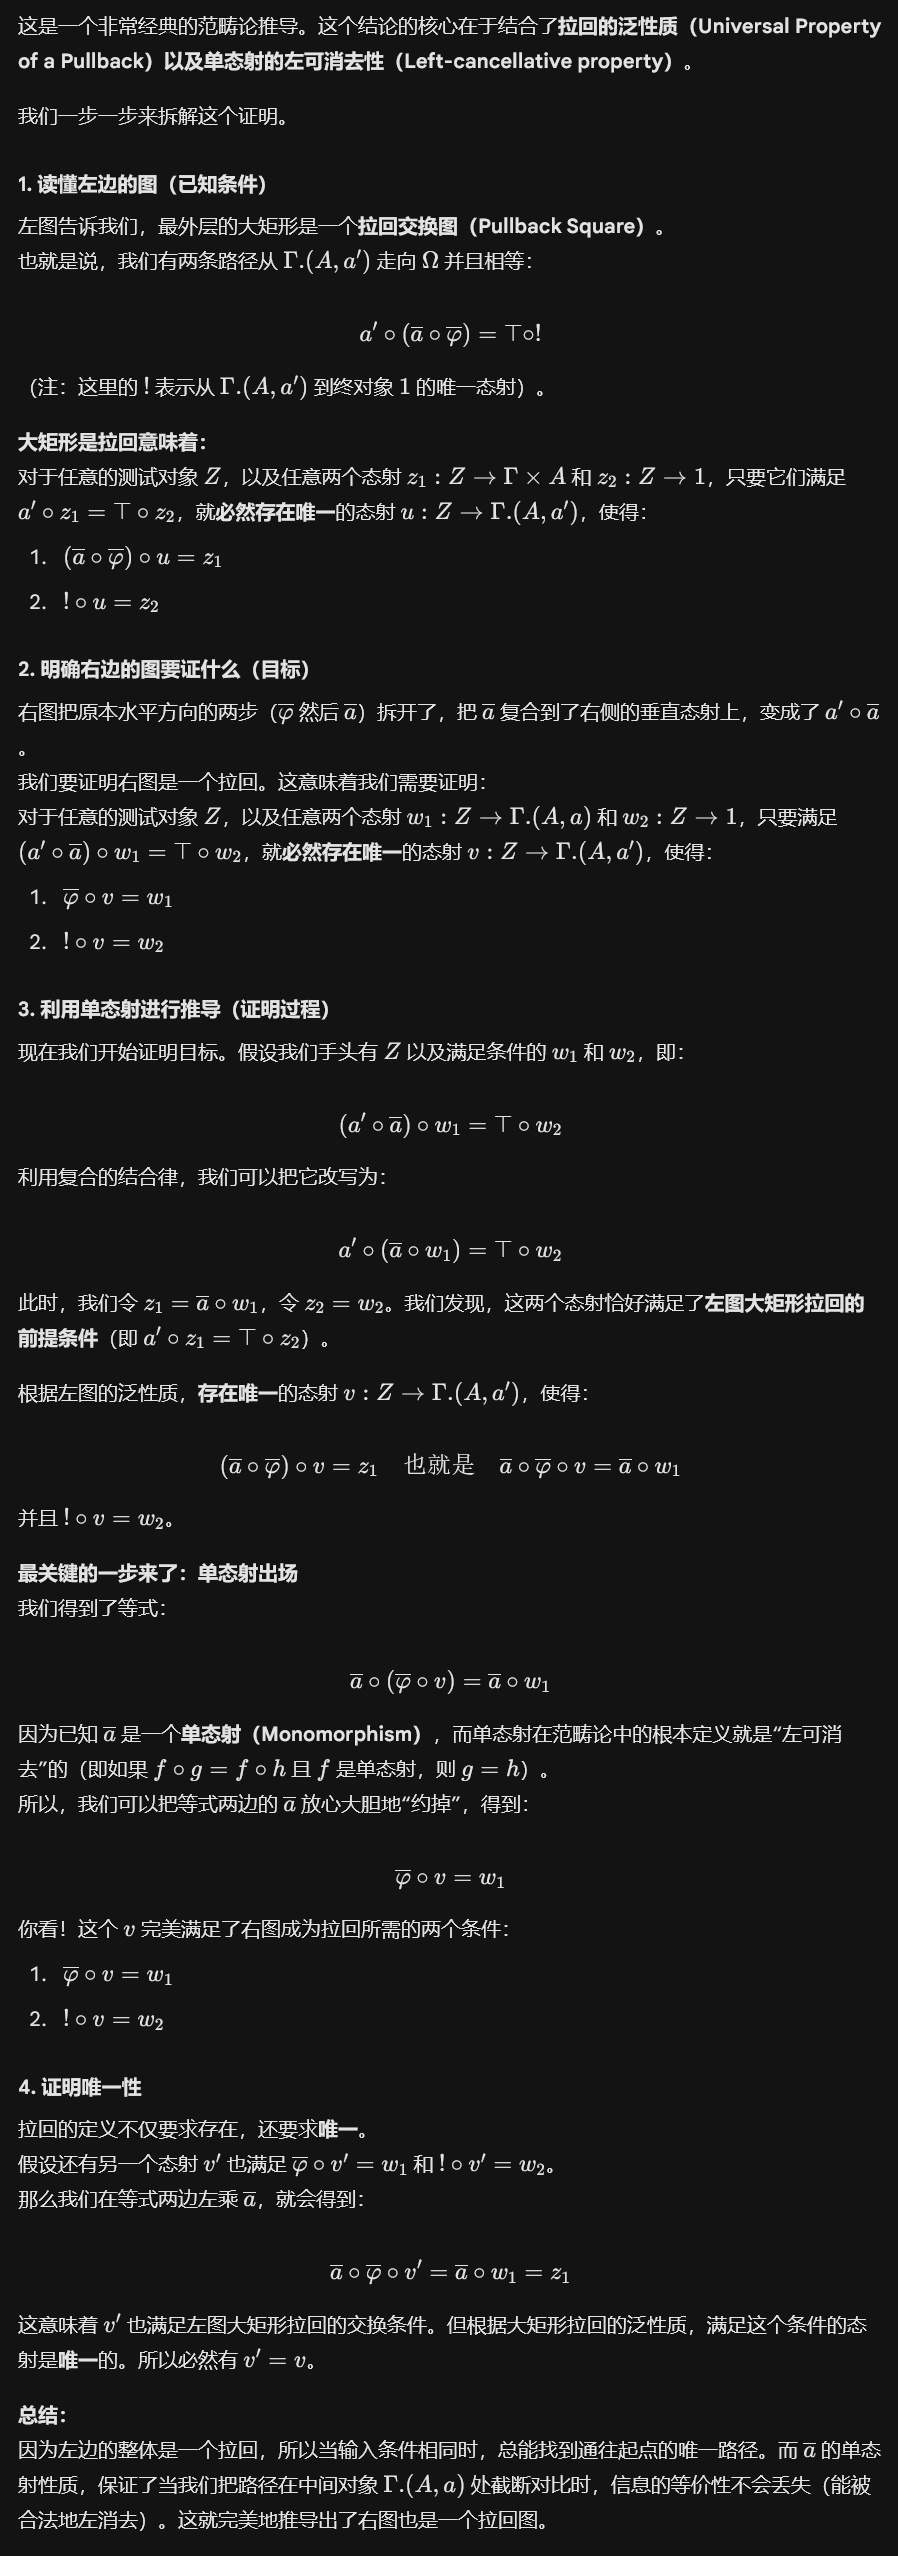
\includegraphics{pullback}
  \end{center}
\end{frame}

\begin{frame}[fragile,shrink]{$\Gamma\vdash\varphi(t)$的分析}
  $\varphi \in \Ter(\Gamma.(A,a)\vdash\Omega) \implies \varphi \in \Ter(\Gamma.(A,a)\vdash(\Omega,\snd))$

  $\varphi : \Gamma.(A,a) \to \Omega$

  $t\in\Ter(\Gamma\vdash(A,a))$

  $\langle id,t\rangle : \Gamma \to \Gamma.(A,a)$

  $\Gamma\vdash\varphi(t):\Omega \implies \varphi(t) \in \Ter(\Gamma\vdash\Omega)\implies \varphi[\langle id,t\rangle] \in \Ter(\Gamma\vdash(\Omega,\snd))$

  $\varphi[\langle id,t\rangle] = \varphi \circ \langle id,t\rangle : \Gamma \to \Omega$

  \[
  \begin{tikzcd}[column sep=huge,row sep=huge]
    \Gamma \arrow[d] \arrow[r,"{(id,\varphi \circ \langle id,t\rangle)}"] & \Gamma\times\Omega \arrow[d,"\snd"] \\
    1 \arrow[r,"\top"] & \Omega
  \end{tikzcd}
  \]
  \begin{align*}
  \snd\circ(id,\varphi \circ \langle id,t\rangle) &= \top\circ1_{\Gamma} \\
  \varphi\circ\langle id,t\rangle &= \top\circ1_{\Gamma}
\end{align*}
\end{frame}

\begin{frame}[fragile,shrink]{$t\in\Ter(\Gamma\vdash(A,a'))$}
  \[
  \begin{tikzcd}
    \Gamma \arrow[d] \arrow[r,"{(id,t)}"] & \Gamma\times A \arrow[d,"a'"] \\
    1 \arrow[r,"\top"] & \Omega
  \end{tikzcd}
  \]
  \[
  a'\circ(id,t)=a'\circ\overline{a}\circ\langle id,t\rangle=\varphi\circ\langle id,t\rangle=\top\circ1_{\Gamma}
  \]
\end{frame}

\begin{frame}[fragile,shrink]{消除规则的合理性$t\in\Ter(\Gamma\vdash(A,a'))\implies t\in\Ter(\Gamma\vdash(A,a))$}
    \[
  \begin{tabular}[t]{lr}
  \begin{tikzcd}
    \Gamma \arrow[r,"{(id,t)}"] \arrow[d] & \Gamma\times A \arrow[d,"a'"] \\
    1 \arrow[r,"\top"] & \Omega
  \end{tikzcd}
&
  \begin{tikzcd}
\Gamma
\arrow[drr, bend left, "{(id,t)}"]
\arrow[ddr, bend right]
\arrow[dr, dotted, "{\langle id,t\rangle}"] & & \\
& \Gamma.(A,a') \arrow[dr,phantom,"{\lrcorner}",very near start] \arrow[r,tail,"{\overline{a'}}"] \arrow[d]
& \Gamma\times A \arrow[d, "a'"] \\
& 1 \arrow[r, "\top"]
& \Omega
\end{tikzcd}
  \end{tabular} \]
  $(id,t) = \overline{a'}\circ\langle id,t\rangle = \overline{a}\circ\overline{\varphi}\circ\langle id,t\rangle$
  \[
  \begin{tabular}{cc}
    \begin{tikzcd}
    \Gamma \arrow[r,"{(id,t)}"] \arrow[d] & \Gamma\times A \arrow[d,"a"] \\
    1 \arrow[r,"\top"] & \Omega
  \end{tikzcd}
  &
  \begin{tikzcd}
  \Gamma\arrow[r,"{\langle id,t\rangle}"] & \Gamma.(A,a')\arrow[r,"{\overline{\varphi}}"] & \Gamma.(A,a) \arrow[r] & 1
  \end{tikzcd}
\end{tabular}
  \]
  $a\circ(id,t)=a\circ\overline{a}\circ\overline{\varphi}\circ\langle id,t\rangle=\top\circ1_{\Gamma.(A,a)}\circ\overline{\varphi}\circ\langle id,t\rangle = \top\circ1_{\Gamma}$
\end{frame}

\begin{frame}[fragile,shrink]{子单元素集}
  在先前的定义中取$A=\bfone$, 我们得到, 对于每一个$\varphi:\Omega$, 存在一个类型, 其“居留性”(即该类型是否拥有元素)对应于$\varphi$的可证明性:
  \[ [\varphi]\triangleq \{\ul:\bfone\mid\varphi\} \]

  如果 $φ$ 是一个全局命题(即在空上下文中定义的命题, 或者一个 $\bfone → Ω$ 的态射)
  \[
  \begin{tikzcd}
    {[\varphi]} \arrow[r,tail] \arrow[d] & \bfone \arrow[d,"\varphi"] \\
    \bfone \arrow[r,"\top"] & \Omega
  \end{tikzcd}
  \]
\end{frame}

\begin{frame}[fragile,shrink]{解释}
严格按照定义来说, 取 $A=\bfone$ 的同时要给出一个态射 $a : \Gamma \times \bfone \to \Omega$
\[
  \begin{tikzcd}
    \Gamma\times\bfone \arrow[r,"!_{\Gamma\times\bfone}"] & \bfone \arrow[r,"\top"] & \Omega
  \end{tikzcd}
\]
$a \triangleq \top\circ !_{\Gamma\times\bfone}$
\begin{comment}
\[
\begin{tikzcd}
  \text{Domain}(\overline{a_{top}}) \arrow[r, "!"] \arrow[d, tail, "\overline{a_{top}}"] & 1 \arrow[d, "\top"] \\
  \Gamma \times 1 \arrow[r, "a_{top}"] & \Omega
\end{tikzcd}
\]
\[
\begin{tikzcd}
  \Gamma \times 1 \arrow[r, "!_{\Gamma \times 1}"] \arrow[d, "id_{\Gamma \times 1}"] & 1 \arrow[d, "\top"] \\
  \Gamma \times 1 \arrow[r, "a_{top}"] & \Omega
\end{tikzcd}
\]
\end{comment}
\[
\begin{tikzcd}
\Gamma.(\bfone,a) \arrow[r,"{\bar{a}}"] \arrow[d] \arrow[dr,phantom,"\lrcorner" very near start] & \Gamma\times\bfone \arrow[d,"a"] \\
\bfone \arrow[r] & \Omega
\end{tikzcd}
\]
可以证明 $\bar{a} = id_{\Gamma\times\bfone}$
\[
  \begin{tikzcd}
    \cdot \arrow[r,tail,"\overline{\varphi}"] \arrow[d] & \Gamma.(\bfone,a) \cong\Gamma\times\bfone\cong\Gamma \arrow[d,"{\varphi}"] \\
    \bfone \arrow[r] & \Omega
  \end{tikzcd}
\]
\end{frame}

\begin{frame}[fragile,shrink]
\[
\begin{tikzcd}
\cdot \arrow[r,"{\bar{a}\circ\bar{\varphi}}"] \arrow[d] \arrow[dr,phantom,"\lrcorner" very near start] & \Gamma\times\bfone \arrow[d,"a'"] \\
\bfone \arrow[r] & \Omega
\end{tikzcd}
\]
\begin{itemize}
\item $\bar{a}\circ\bar{\varphi} = id_{\Gamma\times\bfone}\circ \bar{\varphi} = \bar{\varphi}$
\item 所以$a'$是由$\varphi$直接诱导的
\item $[\varphi] \triangleq (\bfone, a')$
\item $a' \triangleq \varphi\circ p_1$, 其中 $p_1 : \Gamma\times\bfone \to \Gamma$ 是投影态射
\end{itemize}
\end{frame}

\end{document}